
\subsection{Knowledge Graphs}\label{subsec:introduction-knowledge-graphs}

\begin{wrapfigure}{r}{0.5\textwidth} % Float right, width half the text width
    \centering
    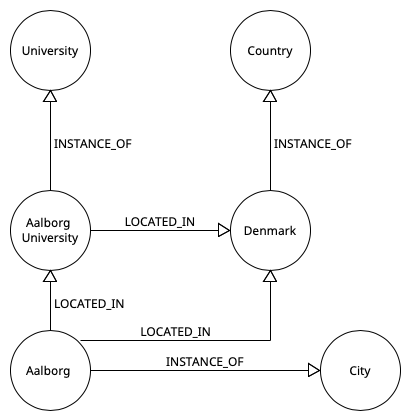
\includegraphics[width=\linewidth, scale=0.5]{figures/kg-example}
    \caption{Example of a knowledge graph.}
    \label{fig:kg-example}
\end{wrapfigure}
While there is no formal, widely accepted definition of Knowledge Graphs, one may think of them as a directed heterogeneous graphs
created with the intent of representing knowledge bases in a machine interpretable manner.

Nodes may (but not bound to) be objects, events, situations, abstract concepts or locations,
with the edges between the nodes representing conceptual relationships among the entities.

Knowledge graphs are often represented as lists of statements such that a statement is: $s = (h,r,t)$
where $h$ refers to the head entity, $t$ represents the tail entity and $r$ represents the
edge connecting the two entities.
These statements have also been called triplets.


Knowledge graphs are often backed by predefined ontologies.
Ontologies define entities and relationships referenced in the list of statements.
serving as their explicit schema, making the parsing of and
work with these graphs easier.

One may also think of knowledge graphs as the combination of the statements, and the relevant ontologies.

Some use cases of knowledge graphs include Google's enhanced contextual response to search queries~\cite{GoogleKnowledgeGraph} (using their internal
knowledge graph) or a more recent example: researchers have been experimenting with augmenting large language models
with knowledge graphs~\cite{LLMKG}, in order to ensure factual answers.

Examples of publicly available knowledge graphs are: Wikidata~\cite{Wikidata} a generic
knowledge graph backing the rest of the Wikimedia ecosystem, or WN18 dataset parsed from WordNet
introduced by~\cite{TransE} and is commonly used to evaluate the performance of various graph machine learning models.



\FloatBarrier
\subsection{Graph Representation Learning}\label{subsec:introduction-graph-representation-learning}
Graph Representation Learning is a research field dedicated to create various methods of embedding nodes of a graph into
a low dimensional vector space that may be used to perform various downstream tasks such as graph and node classification, or link prediction.

These GRL models rely on an encoder-decoder model.
"The intuition behind the encoder-decoder idea is the following:
if we can learn to decode high-dimensional graph information—such as the global positions of
nodes in the graph or the structure of local graph neighborhoods—from encoded low-dimensional embeddings, then, in principle,
these embeddings should contain all information necessary for downstream machine learning tasks"~\cite{RLGMandA}

In other words, while downstream tasks consume the vector representation, the decoder is used to create a well-trained encoder model.

The encoder may create either shallow embeddings, or deep embeddings.
Shallow embedding techniques are generally simpler and faster to train, but
may struggle to capture highly complex patterns and hierarchical relationships within the graph.

Example of shallow embedding methods include: Node2Vec~\cite{Node2vec} or DeepWalk~\cite{DeepWalk}

Deep embedding methods are commonly some variation of Graph Neural Networks detailed in section~\ref{subsec:introduction-graph-neural-networks}

\subsection{Graph Neural Networks}\label{subsec:introduction-graph-neural-networks}
The challenge in creating encoding models that capture deep insight into graph structures, is that graph structures are inherently variable ~\cite{GRLBook}.

For example, if one was to build a model that categorizes social networks using classical tools such as Convolutional Neural Networks or Recurring Neural Networks,
the model would be restricted to graphs with a set amount of nodes.

To address the above issue, and the leverage the structure of graphs Graph Neural Networks are used, which leverage the concept of Neural Message Passing.
The recent state-of-the art knowledge graph completion models are commonly based on some neural message passing framework~\cite{LPSOTA}, due to their inherent ability to capture
deeper neighborhood structures.

\begin{figure}[h] % [h] attempts to place figure here, other options like [t]op, [b]ottom
    \centering % Centers the figure horizontally
    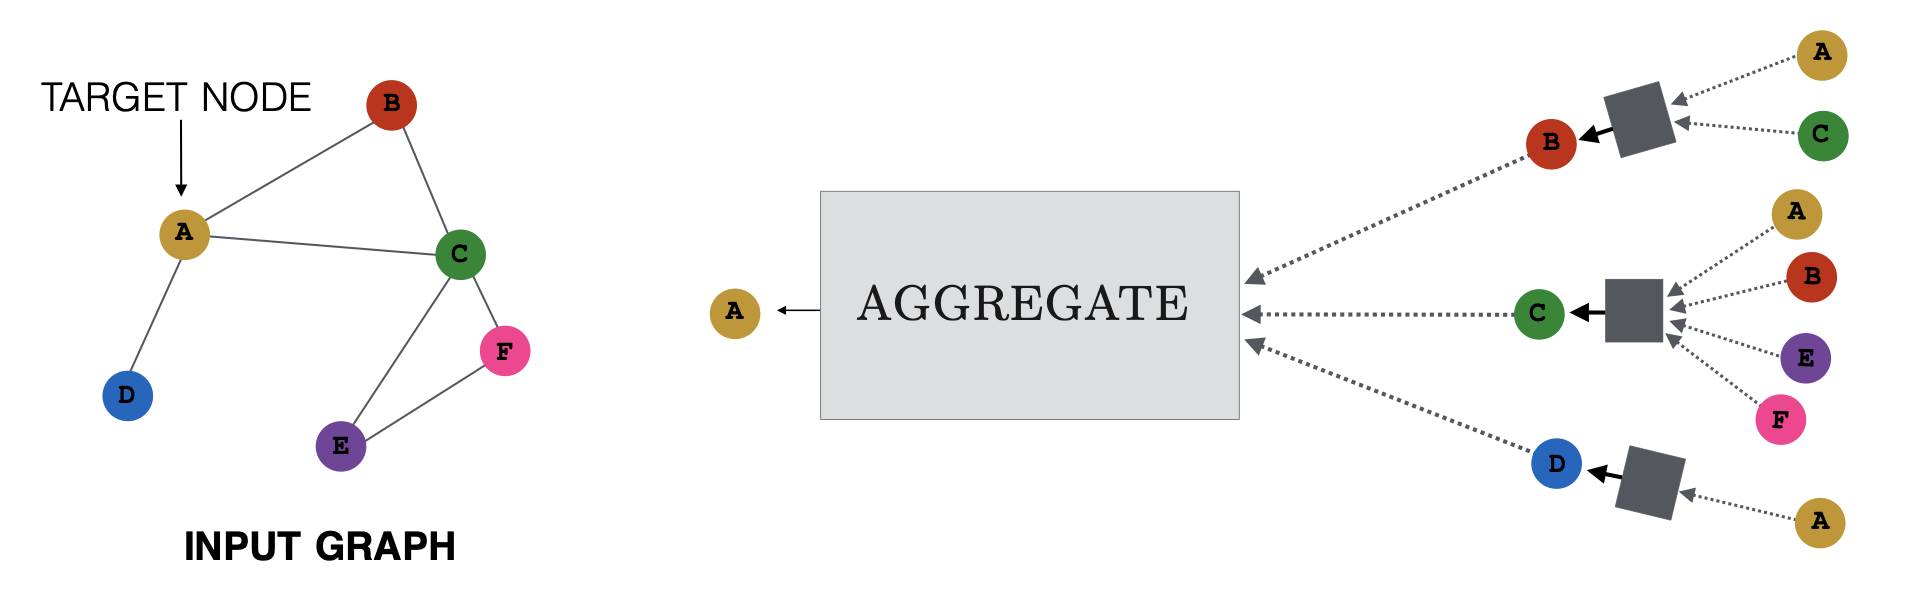
\includegraphics[width=0.9\linewidth]{figures/gnn} % Include the image with desired width
    \caption{A figure from the book, Graph Representation Learning~\cite{GRLBook} showcasing the general intuition behind neural message passing.} % Add a caption
    \label{fig:gnn} % Assign a label for referencing the figure in text
\end{figure}


\subsection{Wikidata}\label{subsec:introduction-wikidata}
"Wikidata is a free, collaborative, multilingual, secondary knowledge base, collecting structured data to provide support for Wikipedia, Wikimedia Commons, the other wikis of the Wikimedia movement,
and to anyone in the world."

"The Wikidata repository consists mainly of items, each one having a label, a description and any number of aliases.
Items are uniquely identified by a Q followed by a number, such as Douglas Adams (Q42).
Statements describe detailed characteristics of an Item and consist of a property and a value.
Properties in Wikidata have a P followed by a number, such as with educated at (P69)."~\cite{Wikidata}

As detailed later in section~\ref{sec:graph-building} the initial dataset that forms the basis of this thesis contains a number of nodes that have inferred Wikidata Ids.
Therefore, Wikidata will be used as a potential source for enriching the dataset, creating a denser network.

Moreover, a secondary object of this thesis is to represent Kitāb Mu'jam al-Buldān in a consumable knowledge graph format.
Therefore, it is easy to argue that using Wikidata's ontology will streamline such efforts.

\subsection{Neo4j}\label{subsec:introduction-neo4j}
During the development stages of this thesis, a heavily used tool was Neo4J~\cite{Neo4j}.
Neo4J is a No-SQL database engine, designed to store and manipulate graph-like structures.
The end user may access and modify the data via Neo4J's custom query language - Cypher.

While other similar graph database engines are available and would have been sufficient, this project uses Neo4J
due to its wide adoption and subsequent easy of access to relevant information.

\subsection{Evaluation Metrics}
This section details the commonly used metrics in link prediction literature.
The usual environment for model evaluation involves the generation of synthetic negative triplets.
These negative triplets, alongside the posit are then ranked based on the score
There are various methods for synthetic negative generation, but in this thesis, a simple corruption
method was used, where either the tail or the head entity is changed in a positive triplet.

This approach is later discussed in section TODO Insert conclusion section.

Notationally, in the next few section $Q$ refers to a set of triples $s = (h,r,t)$ where $s \in Q$~\cite{ampligraph}
\subsubsection{Rank Score}
Simple integer value, the rank of a positive triplet in a vector of negative triplets.

\subsubsection{Mean Rank}
The average rank score of a vector of a positive triplets in $Q$
\[
MR = \frac{1}{|Q|}\sum_{i = 1}^{|Q|}rank_{(h, r, t)_i}
\]

\subsubsection{Mean Reciprocal Rank}
Similar to Mean rank, but instead of averaging triplet ranks, the reciprocal of ranks are averaged.
This should make the metric more robust against outliers ~\cite{ampligraph}

\[
    MRR = \frac{1}{|Q|}\sum_{i = 1}^{|Q|}\frac{1}{rank_{(h, r, t)_i}}
\]

\subsubsection{Hits@K}
The ratio of how many positive triplets make it to the top $K$ list of triplets when ranked against negative triplets.
\[
    Hits@K = \sum_{i = 1}^{|Q|} 1 \, \text{if } rank_{(h, r, t)_i} \leq K
\]
In this thesis $K={1,3,5}$